%*******************************************************************************%
%===================================Information=================================%
%           Author:     Casper van Wezel                                        %
%           Template:   Based on the IEEE template                              %
%                                                                               %
%                       IoT                                                     %
%                       2017-11-16                                              %
%*******************************************************************************%

\documentclass[a4paper,journal]{DDREAM}

% correct bad hyphenation here
\hyphenation{op-tical net-works semi-conduc-tor}
%\usepackage[dutch]{babel} 

\usepackage{import}
\inputfrom{./}{macros}
\newlength\figureheight
\newlength\figurewidth
\usepackage[percent]{overpic}
%\usepackage{siunitx}
%\usepackage{hyperref}
%\usepackage{tikz}
%\usetikzlibrary{arrows,automata,shapes,calc,positioning,decorations.markings}

\newcommand{\paragraphC}[1]{{\bfseries #1: }} % Easy to use bfseries command, with proper brackets


%**********************************************************************************
%=============================Begin Document=====================================%
%**********************************************************************************

\begin{document}
%
% paper title
% can use linebreaks \\ within to get better formatting as desired
\title{\vspace*{0.0cm} Solar Irradiance Prediction \\ using IoT-enabled Solar Modules}
%
%
% author names and IEEE memberships
% note positions of commas and nonbreaking spaces ( ~ ) LaTeX will not break
% a structure at a ~ so this keeps an author's name from being broken across
% two lines.
\author{\vspace*{0.0cm}Anirudh~Bisht~,
Nikolas~Skartsilas,
Casper~van~Wezel,~\IEEEmembership{Delft University of Technology}% <-this % stops a space
\thanks{\footnotesize{This group of Embedded Systems Master students from Delft University of Technology is formed to work togethor on this project.
This report is written as part of the course `Internet of Things Seminar' (IN4398 2016/2017).}}%
}

%--------------------------------------------------------------------------------
% The paper headers
\markboth{\strangesize{IoT IN4398 2016/2017, TU Delft}}%
{C. van Wezel}%
% The only time the second header will appear is for the odd numbered pages
% after the title page when using the twoside option.
%--------------------------------------------------------------------------------
% make the title area
\maketitle


%\boldmath
\begin{abstract}
This paper shows the process of the development of a prototype system representing multiple houses with PV systems where their data is combined in order to ehance current cloud predictions but more importantly to make a short term prediction of PV power generation.
\end{abstract}
% IEEEtran.cls defaults to using nonbold math in the Abstract.
% This preserves the distinction between vectors and scalars. However,
% if the journal you are submitting to favors bold math in the abstract,
% then you can use LaTeX's standard command \boldmath at the very start
% of the abstract to achieve this. Many IEEE journals frown on math
% in the abstract anyway.

\begin{IEEEkeywords}
Internet of Things, IoT, Solar, Solar Modules, Irradiance Prediction, Solar Power Prediction, Microgrid Prediction
\end{IEEEkeywords}

\section{Introduction}\label{sec:introduction}
\IEEEPARstart{T}{here} are a more and more photovoltaic systems deployed world wide every day.
This is all done with the mindset to harvest as much solar energy as possible in order to provide a sustainable electricity source for our increasing needs.
Experts in this area see it as a real posibility that in the future our energy grid will be based on a lot of smaller electricity sources like these home PV systems, the so called micro-grid.
One of the main drawbacks of these micro-grid is controllability, because of the sheer number of contributers.
Currently there is a lot of rotating mass connected to the energy grid (because of all the heavy metal turbines), tinny fluctuations in the power flow of the grid are smoothened by this energy buffer.
Bigger fluctations are controlled by the network operator by increasing or decreasing the power generator at the different sites.
Keeping this in mind, a big disadvantage can be seen when looking back at the home PV systems.
To start with, there will be almost no inertia in a micro-grid system and on top of that the power generation is heavily dependent on the current irradiance by the sun and cloud movement.
So this method of generating energy is way less controllable and also really unpredictable.
This proposes some challenges in the future development of the power grid.

Another major drawback of current photovoltaic systems is the great impact of partial shading of a panel on the whole system.
Because all the cells are connected in series, a smaller generated current in one cell decreases the current through all cells.
A lot of research is done in this area to solve this not so well known problem, all possibilities are discussed in \cite{SoCeBa}.
The authors of this thesis also propose and design an implementation to solve this problem.
In general, most implementations use a microcontroller which optimizes the power output in someway.
With current trends of all devices being more and more connected to the internet (the Internet of Things era), this might also provide the possibilities to provide a solution for the problem of the predictability of micro-grid PV systems.

In the future, all the PV modules will be 'smart' (i.e. have a microcontroller in them), this can be used to collect huge amounts of data of the current irradiance.
Using all this data and the geographical locations, the resolution of cloud movement predictions can be enhanced greatly.
These more accurate cloud predictions or models can be fed back into the system in order to make a short term prediction of the power generation of these small PV systems.

In this report the future problems mentioned above will be further explained in \bigref{sec:problem_definition}.
The algorithm designed to the prediction and the simulation to verify it are explained in the \nameref{sec:implementation} part.
The different subparts of the test setup are explained in \nameref{sec:experiment} after which some reflections on this project are made and some conclusions are drawn.

\section{Problem Definition}\label{sec:problem_definition}
\IEEEPARstart{T}{o} smoothen the effect of the unpredictability of the sun and cloud on a solar based power grid, we need to have a network of communicating nodes. This communication will facilitate cloud prediction algorithms to be run that will allow these nodes to be more prepared for power fluctuations. The goal is to create an algorithm that will pool that from each node and provide a prediction to the nodes of the cloud coverage. In addition to the algorithm we also show a hardware implementation to showcase the working implementation of the algorithm.

\section{Implementation}\label{sec:implementation}
\IEEEPARstart{A}{s} the main purpose of this research is to show the viability of the proposed prediction method, the designed algorithm is explained in the next section.
This algorithm is tested using simulation data generated by the simulator explained afterwards.

\clearpage

\subsection{Algorithm}\label{sec:implementation-algorithm}
Cloud predictions currently uses complex weather models because of their many variables and big simulation area these simulations are really computationally intensive.
Meteorology instutes often have supercomputers with 10s or 100s thousand of cores.
When this application would be used in a full scale or real world setting, algorithms can of course use differential equations or machine learning.
However because we are keeping the number of nodes relatively low, equally spaced and are using a controlled test setup, many simplifications can be done to the algorithm to the point where just a simple loop can be used.
Inside this loop, the correlation between the different time domain signals measured at the different houses can be found.
When there is a correlation between these signals, it can be stated that the same cloud was above both nodes.
This correlation can be implemented using a convolution, the location of the highest peak gives the time difference between the signals.
This time difference is the key towards prediction of course.
All the different arrival times can be fitted, using this fit a prediction can be made.

In \autoref{fig:flowchart} this algorithm is shown using a flowchart, a small remark is made for each step.

\paragraphC{get samples} First the Raspberry Pi is given the command to ask all the I2C slaves (i.e. the houses) for their ADC samples.
Using a threshold value, this is converted to a binary value indicated shaded or not.

\paragraphC{cloud detection} The data is checked to see if a cloud has appeared.

\paragraphC{Get Cloud Shape} When a cloud is found, the time domain signal of this cloud at the house where it is first detected will be selected as the reference shape.

\paragraphC{Find Correlation} Using this cloudShape, a loop finds all the correlations between this shape and the data of the other houses.

\paragraphC{Find Peaks} The location of the peaks in the correlations tells the delay between the 2 signals.
Because the start time of the first cloud is known, the arrival times can be calculated.

\paragraphC{Fit Arrival Times} All these arrival times can be fitted.

\paragraphC{Extrapolate Fit} Extrapolating this fit, gives a prediction for the arrival time of the cloud at another house (i.e. ETA).

\paragraphC{Send ETAs} These ETAs are send back to the RPi, so it can warn the nodes about upcomming clouds (the nodes will then change their LED Status).

\begin{figure}[H]
\centering
    \subimport{resources/}{flowchart.tikz}
    \caption{Flowchart of the prediction algorithm}
    \label{fig:flowchart}
\end{figure}

\subsection{Simulation}\label{sec:implementation-simulation}
To test the prediction algorithm, some validation data was needed.
To easy the process of troubleshooting this is done best by using a simulation which can be wrapped around the prediction algorithm.
The basic function of this simulation is to generate clouds and store the data.
To accomodate multiple different scenarios everything is parametrized.
Which means that it is easy to change the grid size, the number of houses in each direction of the grid, both cloud dimensions, cloud origin, cloud speed and of course the number of Simulation Steps.
The data is saved to a \texttt{.mat} file and also visuallized in plots, these frames are also combined to into a \texttt{.gif}.
Below some different simulation frames are shown.

\begin{figure}[H]
\centering
    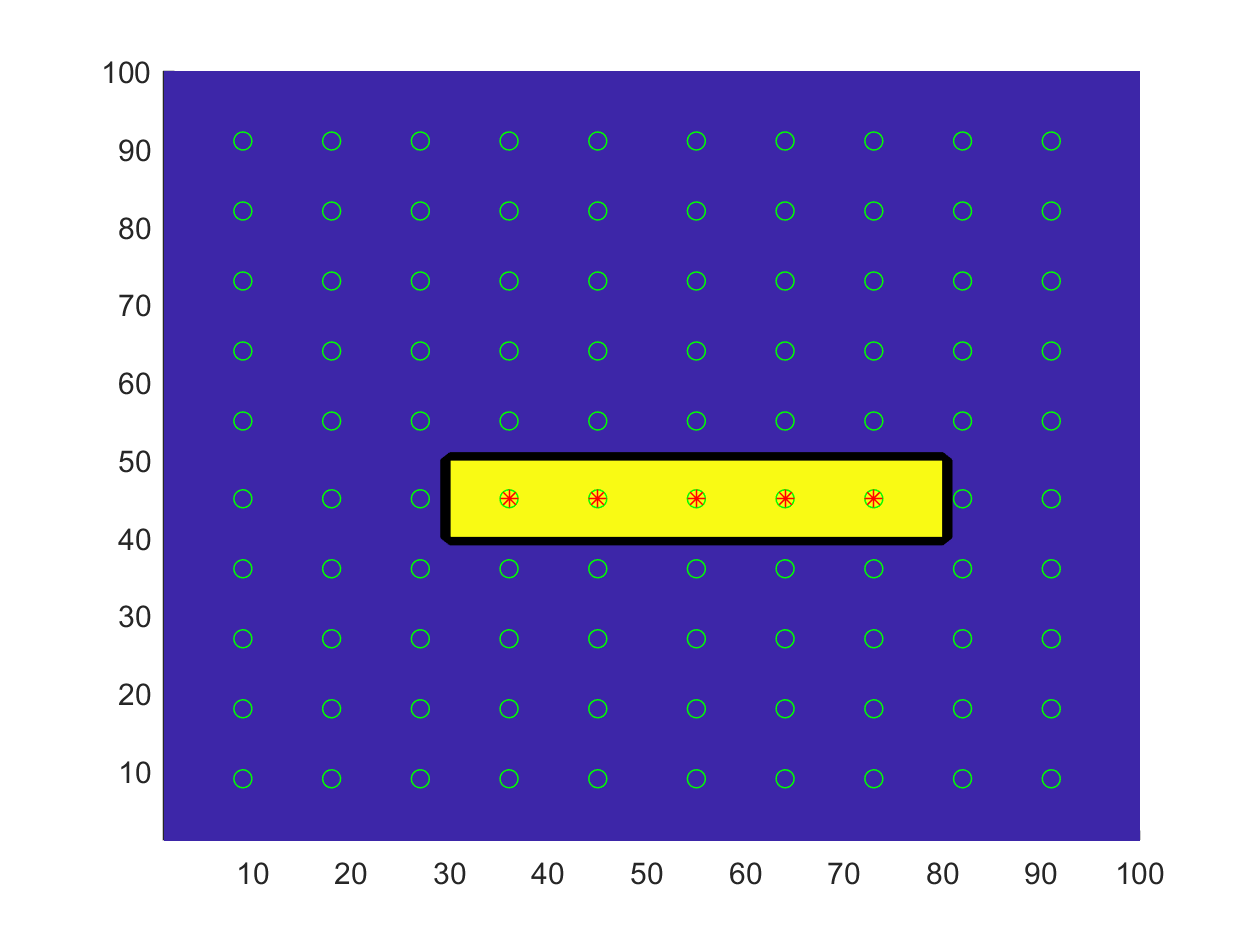
\includegraphics[width=0.5\textwidth]{./resources/10x10-large.png}
    \caption{simulation of 10x10 houses with a long cloud}
    \label{fig:sim-10}
\end{figure}

\begin{figure}[H]
\centering
    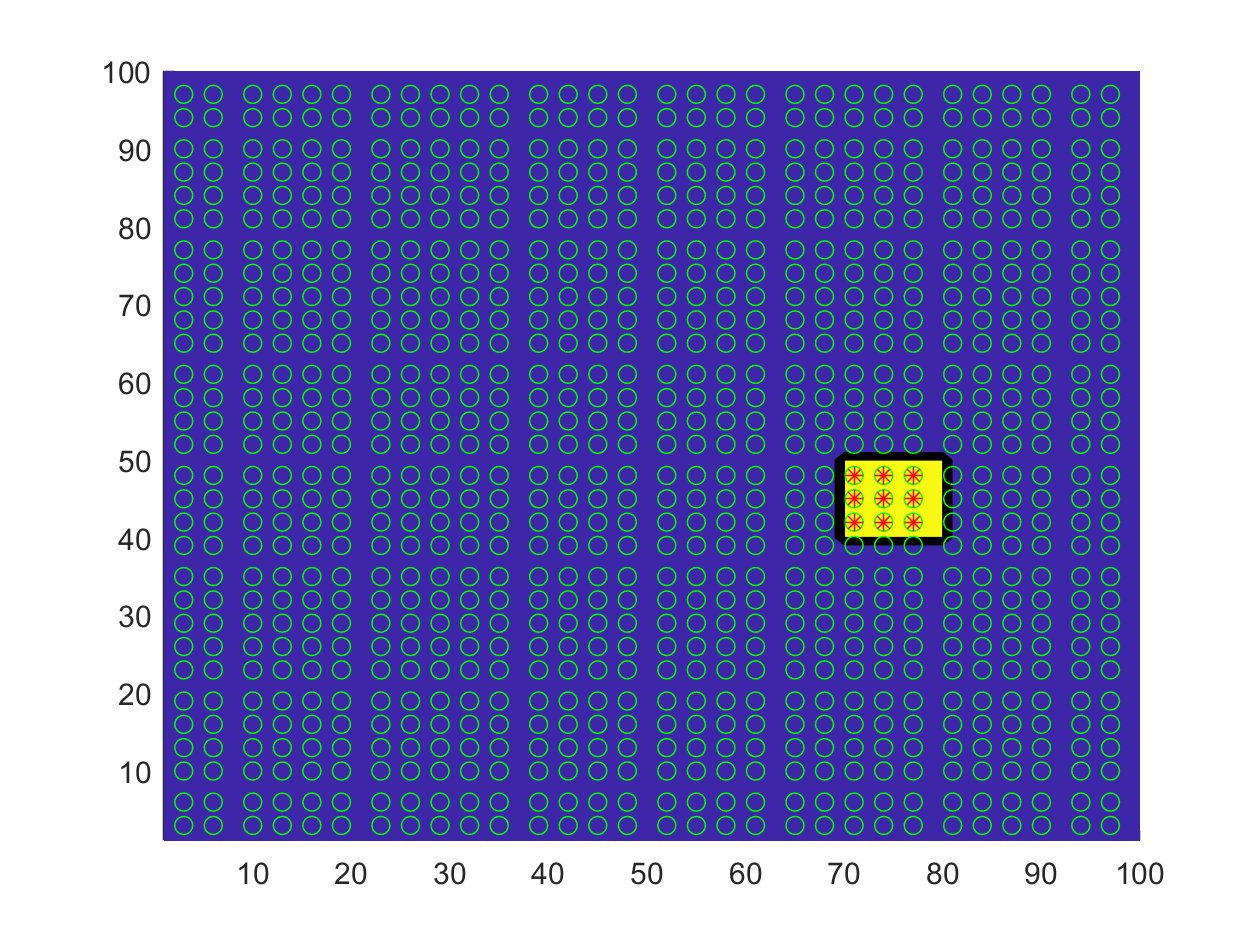
\includegraphics[width=0.5\textwidth]{./resources/30x30.png}
    \caption{Simulation of 30x30 houses with a small cloud}
    \label{fig:sim-30}
\end{figure}

\begin{figure}[H]
\centering
    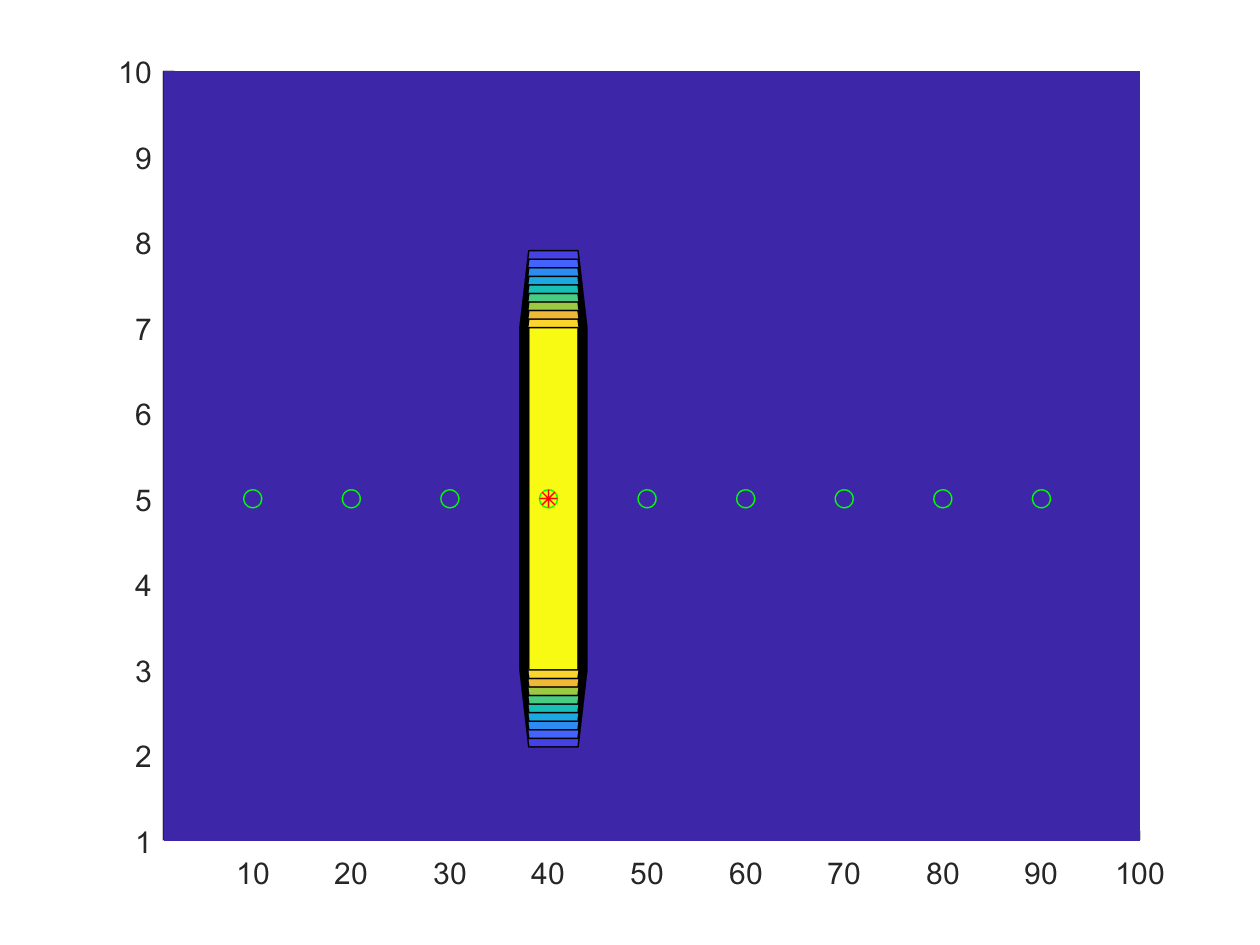
\includegraphics[width=0.5\textwidth]{./resources/9x1.png}
    \caption{Simulation of 9x1 houses}
    \label{fig:sim-9}
\end{figure}

\section{Experimental Setup}\label{sec:experiment}
\IEEEPARstart{T}{he} goal of this experiment is to provide a prototype showing that this method could work in the future.
The main goal of this Experimental Setup thus is to just show the working version of the algorithm.

\subsection{Hardware}\label{sec:implementation-hardware}
Because the main goal of this prototype is to show that the algorithm works, a lot of simplifications can be made on the hardware level.
The next sections discuss different subparts of the hardware implementation.

\subsection{Nodes}
In real-life this future system would consist of many nodes connected to a network.
These can be either single smart modules, or the data of the panels can already be merged by the MPPT and inverter of the system, which can act as a gateway to the network.
For this prototype, there are barely any requirements regarding the microcontroller.
It should just have at least 1 ADC channel for the sensor and a method for communication.
To save on costs, a bunch of cheap Arduino Nano's from ebay are used.
To demonstrate the prototype, we will just use 9 nodes, in case this all works fine and there is more time, we already have the hardware for 25 nodes.

\subsection{Sensor}
The main feature of the node will be to measure the irradiance seen at that node.
In the real-life system, this will be done by simply measuring the voltage and current and multiplying the to get the output power.
Using the specifications of the panel, this directly results in the irradiance level.
However, because solar panels would be the biggest part of the BOM, some simplifications would be nice.
There are multiple sensor to measure irradiance, for example photodiodes and Light Dependent Resistors (LDRs).

Photodiodes are really fast and accurate, however reading their output value can be quite tricky.
LDRs on the other hand can just be used in a simple voltage divider, and since we just need to make a distinction between shaded or clear view, consistency and calibration does not really matter.

In order to check the difference, we did a comparision test with 3 PV modules and 3 LDRs by measuring their output over the period of a few days next to an attic window.
See \autoref{fig:sensors} and \autoref{fig:sensors-zoom}

\begin{figure}[H]
\centering
    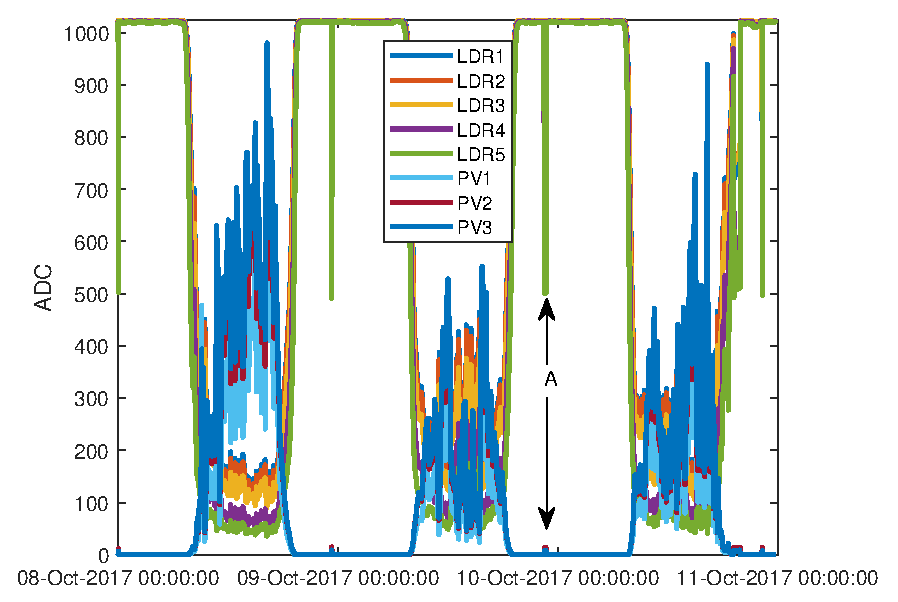
\includegraphics[width=0.5\textwidth]{./resources/sensors.eps}
    \caption{A three day comparison of 5 LDRs and 3 PV modules}\label{fig:sensors}
\end{figure}

\begin{figure}[H]
\centering
    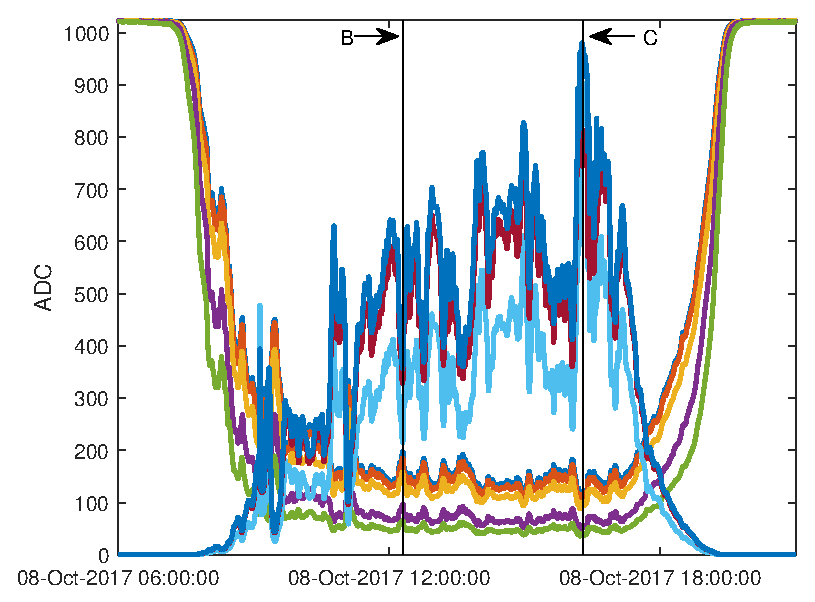
\includegraphics[width=0.5\textwidth]{./resources/sensors-zoom.eps}
    \caption{One day selection of \autoref{fig:sensors}}\label{fig:sensors-zoom}
\end{figure}

Of course the output of the PV modules decreases when shaded and because the LDR was put in the bottom part of the voltage divider, and its resistance decreases with more irradiance, the output is high when shaded.
So when looking at the two different groups, the parabolic shape of the sun intensity throught the day can be clearly seen.
Also the correlation is quite obvious, when the PV outputs drop because of a cloud, the LDR output values increase (see \autoref{fig:sensors-zoom} annotation \emph{B} for a cloud and \emph{C} for a high irradiance peak).
The spikes during the night, e.g. \emph{A} in \autoref{fig:sensors}, are caused by the attic light being turned on.
As a last remark it can be clearly seen that two of the LDRs have a different offset compared to the other 3.
This is due to two different resistors being used in the voltage divider.
The tree LDRs using the \SI{2.2}{\kilo\ohm} resistors (as opposed to the other 2 \SI{4.7}{\kilo\ohm}) gives a bigger fluctation difference, making it easier to detect clouds, so this value will be used in the final setup

\subsection{Network}
In the real-life system, connection all the PV systems of a country would be a challenge.
However with the current trends in IoT and Big Data, this would be no problem in the future.
Different network architectures all have their own benifits of course.
To just name a few, one can simply connect it to the wired internet that is usually already present in the house.
This would be quite cheap, however connecting all IoT devices this way would fill this quite fast.
Current wireless developments such as LoRa prove a nice alternative, as it is specifically designed for IoT applications.
In this prototype setup, something more simple can be used such as I2C.

\subsection{System Integration}
As the main server in this system, a Raspberry Pi is used because of its perfect of this application since it has a full Linux OS and multiple connectivity interfaces.
To first test the basic setup functionality, a Python script was created that runs on the Pi and sends and receives data over the I2C bus.
The algorithm however runs in \matlab, this gap can be filled by forming a file stream communication between the two scripts or generating executable code from \matlab that can be run in a python environment.
However, \matlab offers a really good solution for this with their `Hardware Support Packages'.
After installing the package for your specific hardware platform as an Add-On to your \matlab, you get almost full control over the hardware platform directly from within \matlab running on your computer.
(\matlab supports many different hardware platforms like Raspberry Pi, Arduinos, Lego but also many instrumentation devices.)
Using this package, communicating with the different nodes was as easy as just using \texttt{read} and \texttt{write} to the node address from within \matlab.


\begin{figure}[H]
\centering
    \subimport{resources/}{system.tikz}
    \caption{Block diagram showing the top level system overview}
    \label{fig:system}
\end{figure}

For the Arduino Nano, a header is designed that has the LDR, but also 3 LEDs (Green, Orange, Red) which can be used as status indicators, also the I2C connections are on this header.
The schematic of the header can be seen in \autoref{fig:schematic}, the soldered hardware looks like \autoref{fig:header}.

\begin{figure}[H]
\centering
    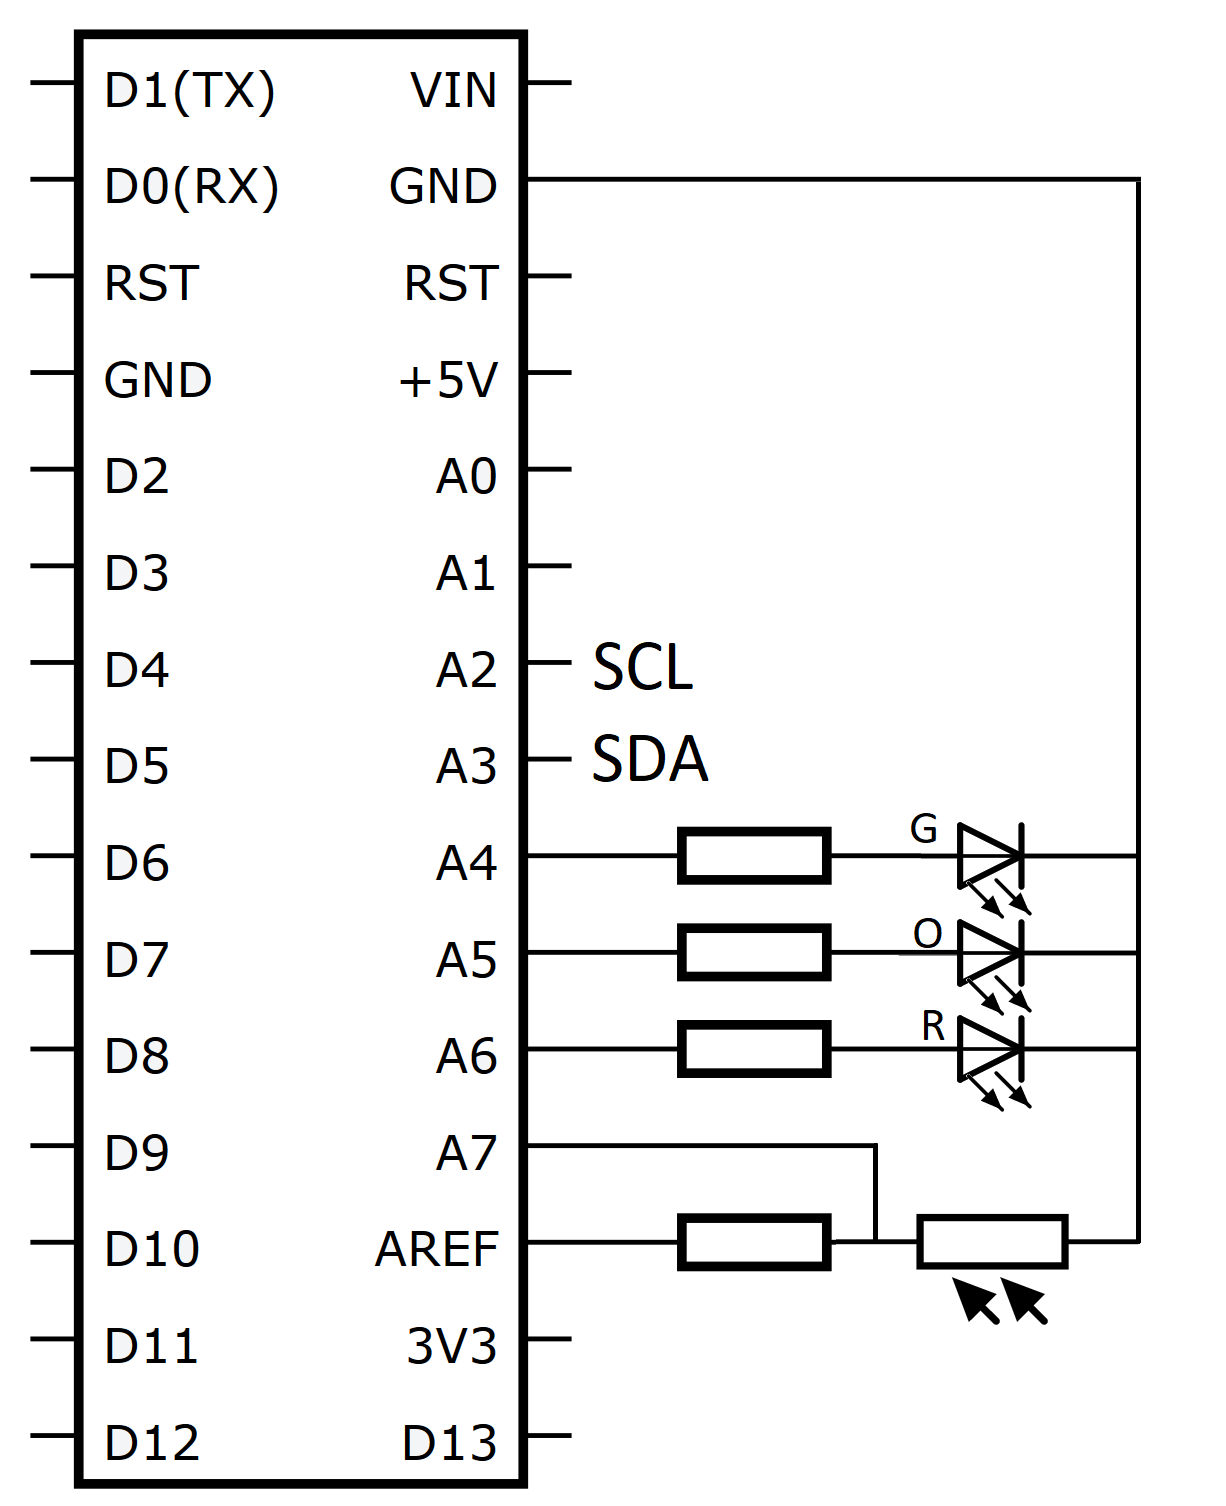
\includegraphics[width=0.35\textwidth]{./resources/schematic.png}
    \caption{Schematic of the header}
    \label{fig:schematic}
\end{figure}

\begin{figure}[H]
\centering
    \includegraphics[width=0.40\textwidth]{./resources/header_closeup.png}
    \caption{Closeup of header}
    \label{fig:header}
\end{figure}

\begin{figure}[H]
\centering
    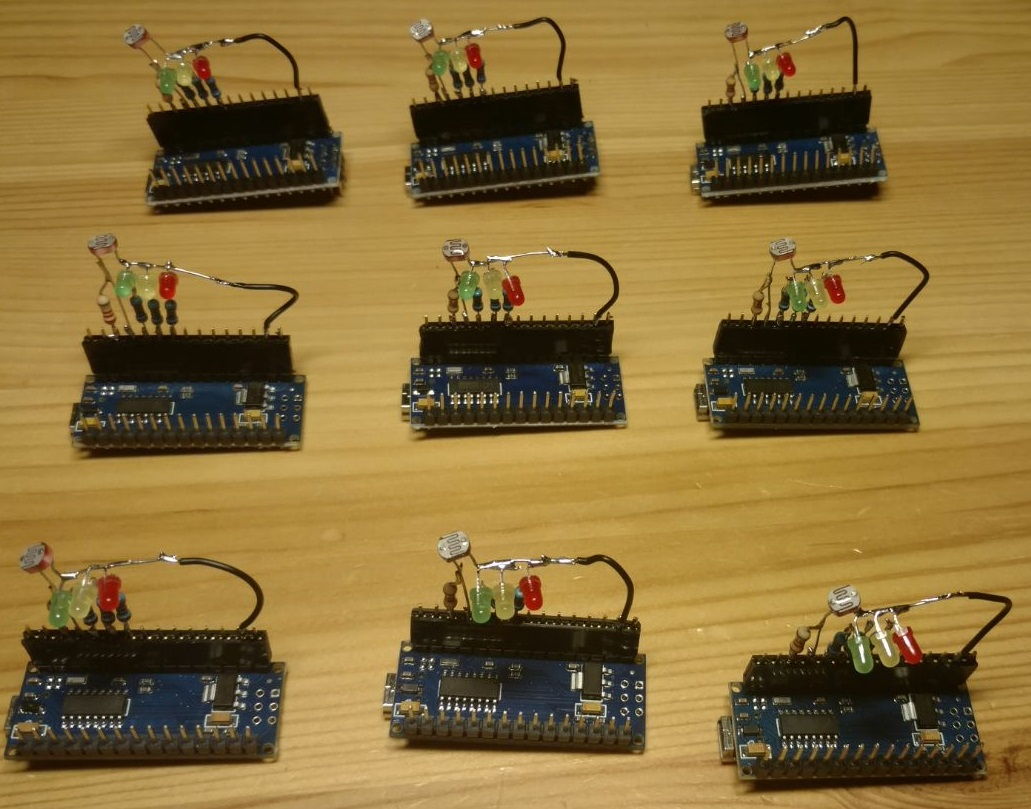
\includegraphics[width=0.45\textwidth]{./resources/nanos.jpg}
    \caption{9 of the Nanos with their headers.}
    \label{fig:nanos}
\end{figure}

\vspace{1cm}
\section{Discussion}\label{sec:discussion}
\IEEEPARstart{R}{eflecting} back on this project there are two different perspectives that can be taken.
The first perspective is of course directly looking at the success and achievements of this project.
This would give quite a positive view, we managed to get a working prototype to show the solution we first proposed.
The other perspective would be from a more negative side, judging the quality of the project.
However when giving critique on this, one has to bear in mind the short time period of this project as well as the available resources.
Money wise there were no limitations, because the price for one house/node is around 2 euros.
However time and knowledge were more critical, since we all three are Embedded Systems students we did not have any knowledge or experience in the mathematical aspects of pattern recognition and prediction.
If one wants to make a full scale version, a first step could be a bachelor graduation project at computer science.

There were no big technical problems throughout this project.
Of course every project has its challenges, but all of those were solved.
The main problems are what now are the conditions for a succesfull prediction.
Initially we wanted 3x3 houses and we had the hardware for an extension to a 5x5 grid.
But making the algorithm spatially independent was too difficult, so we simplified the setup to a linear row of houses.
This directly solved the relatively large number of houses the algorithm need in order to start the prediction.
This is because we use the most basic form of prediction, being just a fit and extrapolation.

\section{Conclusion}\label{sec:conclusion}
\IEEEPARstart{I}{t} can indeed be concluded that the proposed solution can indeed help solving future problems in the power grid.
As can be seen in the video \footnote{\url{https://goo.gl/uQje52}}, the idea of the solution is well demonstrated with this prototype.
Most of the houses are needed to make a proper fit to base the prediction on, but it can be seen that at the last two houses, the LED warning are spot on.
So in order to succesfully use this solution, more work needs to be done to efficiently scale up the algorithm starting of by making proper models and using excisting cloud simulation software.

%\appendices
%\section{Proof of the First Zonklar Equation}
%Appendix one text goes here.

% you can choose not to have a title for an appendix
% if you want by leaving the argument blank
%\section{}
%Appendix two text goes here.


%\section*{Acknowledgment}

% Can use something like this to put references on a page
% by themselves when using endfloat and the captionsoff option.
\ifCLASSOPTIONcaptionsoff
  \newpage
\fi

% trigger a \newpage just before the given reference
% number - used to balance the columns on the last page
% adjust value as needed - may need to be readjusted if
% the document is modified later
%\IEEEtriggeratref{8}
% The "triggered" command can be changed if desired:
%\IEEEtriggercmd{\enlargethispage{-5in}}

% references section

% can use a bibliography generated by BibTeX as a .bbl file
% BibTeX documentation can be easily obtained at:
% http://www.ctan.org/tex-archive/biblio/bibtex/contrib/doc/
% The IEEEtran BibTeX style support page is at:
% http://www.michaelshell.org/tex/ieeetran/bibtex/
%\bibliographystyle{IEEEtran}
% argument is your BibTeX string definitions and bibliography database(s)
%\bibliography{IEEEabrv,../bib/paper}
%
% <OR> manually copy in the resultant .bbl file
% set second argument of \begin to the number of references
% (used to reserve space for the reference number labels box)

\begin{thebibliography}{1}

\bibitem{SoCeBa}
E. de Haan; R. Plaisant van der Wal, C. van Wezel, R. Zwetsloot, \emph{Solar Cell Balancing}. BSc. Electical Engineering Thesis, Delft University of Technology, 2016.

\end{thebibliography}

\end{document}
